%!TEX encoding = UTF-8 Unicode
\documentclass[UTF8, a4paper, 11pt, oneside]{ctexbook}

% 颜色,图像
\usepackage{color, graphicx}
\usepackage{tikz}

% 参考文献,按照被引先后排序
\bibliographystyle{unsrt}

% 索引
\usepackage{makeidx}
\makeindex

% 使用Courier New作为等宽字体
\renewcommand\ttdefault{pcr}

% 源码高亮环境
\definecolor{gray}{rgb}{0.9,0.9,0.9}
\usepackage{listings}
\lstset{
	language=Java, 
	basicstyle=\ttfamily\small, 
	keywordstyle=\color{blue}, 
	commentstyle=\color{darkgreen}, 
	stringstyle=\color{red}, 
	backgroundcolor=\color{gray},
	frame=single,
	numbers=left, 
	numberstyle=\tiny,
	stepnumber=1,  
	xleftmargin=-1em,
	xrightmargin=-3em, 
	aboveskip=0em,
	tabsize=4,
	breaklines=true, 
	title=\lstname,
	extendedchars=false,	% 必须如此,否则和hyperref冲突,出错。
 }

% 页码、页眉风格
\pagestyle{plain}

% 内部引用超链接
\usepackage[pdftex,unicode,colorlinks=true,urlcolor=blue,linkcolor=blue,citecolor=blue]{hyperref}

\begin{document}
\frontmatter
\title{Android恶意代码分析}
\author{肖梓航}
\date{}
\maketitle

\vfill
\thispagestyle{empty}
\begin{center}
\it{To qiyang.}
\end{center}
\vfill

%!TEX encoding = UTF-8 Unicode
\chapter{前言}
毫无疑问,Android平台已经成为恶意代码新的肆虐之地。AVer与VXer的长期对抗将在这一平台延续,正如在PC上一样。而双方人员数量上的显著差异也会长期存在。为了在这个天平的AV这边增加砝码,作者认为有必要将这些技术梳理并公开。最后也就形成了这本小册子。

在这个领域,任何技术都是双刃剑。这本小册子中的技术既可以被安全工作者用于反病毒和软件保护,也可以被攻击者用于病毒对抗和软件破解。如何使用,只在乎人心。而我们应该遵循最自然的道德观,利用这些技术造福于周围的人们。

这本册子中必然有很多错误,更有很多不足之处。如果您有任何建议、看法、意见,希望能告诉我,邮箱是:

\begin{center}
\href{mailto:xiaozihang@gmail.com}{xiaozihang@gmail.com}
\end{center}

或者到本书的项目主页Issue中讨论,地址是:

\begin{center}\href{http://code.google.com/p/amatutor}{http://code.google.com/p/amatutor}
\end{center}

\tableofcontents
\setcounter{tocdepth}{3}

\mainmatter
%!TEX encoding = UTF-8 Unicode
\chapter{静态分析}
\section{apk文件格式}
Android系统使用的安装包文件后缀名为.apk。实际上它是标准的ZIP格式文件,可以使用7-zip等压缩软件、zlib等函数库进行处理
\footnote{ZIP格式的详细介绍,参考\url{http://en.wikipedia.org/wiki/ZIP\_(file\_format)}。}。

一个.apk文件解压缩后,通常包括如下文件或文件夹:
\begin{itemize}
	\item[-] AndroidManifest.xml:项目配置文件,但不是明文的XML文件,直接打开无法阅读
	\item[-] classes.dex\index{classes.dex}:所有的Java类文件被打包并转换为这个文件,它是Dalvik虚拟机上的可执行二进制文件,Android系统在运行时将其动态优化为.dey文件并投入一个Dalvik虚拟机实例中运行。
	\item[-] resources.arsc:资源文件打包而成,字符串值(源码中res/value/Strings.xml)就在其中
	\item[-] res/:资源文件夹,其中包括布局文件夹layout、图标图片文件夹drawable、原始文件文件夹raw(该目录下任何文件都会原封不动地存储到设备上)等
	\item[-] META-INF/:数字签名文件夹
	\item[-] lib/:包含NDK开发中使用的动态链接库文件(ARM架构下ELF格式.so文件),有的软件没有这个文件夹
	\item[-] assets/:原始文件文件夹,其中的文件不会被压缩,也不能想res/目录下的资源文件一样通过R类引用,有的软件没有这个文件夹
\end{itemize}
其中,数字签名文件夹META-INF/包含下列文件:
\begin{itemize}
	\item[-] CERT.SF:生成每个文件相对的密钥
	\item[-] MANIFEST.MF:数字签名信息
	\item[-] xxx.SF:这是 JAR 文件的签名文件,xxx标识了签名者
	\item[-] xxx.DSA:对输出文件的签名和公钥
\end{itemize}

\section{XML解码}
\subsection{AXMLPrinter2}
Android使用了大量XML文件用于项目配置、布局、文本资源等。XML具有较高的可读性,但格式解析的开销较大,适合开发人员编写,但不适合“寸土寸金”的手机解析。因此,Android在编译时将XML文件编码为另一种格式,并使用更快的算法解析格式。编码后的XML文件无法直接阅读。

AXMLPrinter是开源项目android4me\footnote{\href{http://code.google.com/p/android4me/}{http://code.google.com/p/android4me/}}的一个产品,可以将上述编码过程逆向执行,即将编码后的XML文件还原为可读形式。它的使用非常简单:
\begin{lstlisting}[language=bash, numbers=none]
java -jar AXMLPrinter2.jar encoded.xml >decoded.xml
\end{lstlisting}
\section{DEX反汇编}
\subsection{smali}
apk文件中的“代码”实际上都存储在了classes.dex文件之中。这个文件类似于Java的类文件,是Dalvik虚拟机上的二进制可执行文件。smali和下一节介绍的dedexer是两款逆向.dex文件的工具,输出可读性较好的Dalvik指令文件。

smali\footnote{\url{http://code.google.com/p/smali/}}实际上由两个工具smali.jar和baksmali.jar组成。其中,baksmali.jar用于反汇编:
\begin{lstlisting}[language=bash, numbers=none]
java -jar baksmali.jar classes.dex -o dir
\end{lstlisting}
上述命令会在dir目录下输出classes.dex的反汇编结果,其中文件扩展名为.smali,每个Java类一个文件,并以Java package名来组织路径。例如,com.example.Hello类将生成com/example/Hello.smali文件。

smali.jar则用于将.smali文件再次编码为.dex文件:
\begin{lstlisting}[language=bash, numbers=none]
java -jar baksmali.jar dir -o classes_new.dex
\end{lstlisting}

因为精确地汇编与反汇编,smali成为Android病毒编写和分析中最常用的工具之一。
\subsection{IDA}
\subsection{dedexer}
dedexer\footnote{\url{http://sourceforge.net/projects/dedexer/}}是另一个.dex文件反汇编工具,用法是:
\begin{lstlisting}[language=bash, numbers=none]
java -jar ddx.jar -d dir classes.dex
\end{lstlisting}
如果使用\lstinline!-o!参数,还将在dir目录下输出名为dex.log的.dex解析日志。
\section{DEX反编译}
\subsection{dex2jar}
dex2jar\footnote{\url{http://code.google.com/p/dex2jar/}}将classes.dex逆向为Java的类文件(.class文件),并打包为.jar格式。jar格式本质上就是按package路径的类文件的ZIP压缩。

dex2jar并不直接使用classes.dex,它自带了解包功能,命令为:
\begin{lstlisting}[language=bash, numbers=none]
dex2jar Example.apk
\end{lstlisting}
即直接作用于apk文件,在当前目录生成名为Example.apk.dex2jar.jar的文件。

应当注意的是,dex2jar工具的逆向并不完全精确。目前已知在转换switch、try-exception等函数结构时,将会出错。
\subsection{jd-gui}
jd-gui\footnote{\url{http://java.decompiler.free.fr/?q=jdgui}}是一个图形界面的Jar文件反编译器。我们通常用jd-gui来反编译dex2jar产生的.jar文件,得到Java代码。

dex2jar对部分函数结构的逆向错误将直接在jd-gui的反编译结果中显示出来。此外,部分特殊优化的类方法(函数),jd-gui的反编译将失败。
\subsection{ded}
\subsection{soot}
\subsection{undx}

\section{ARM分析}
\subsection{IDA}
除了classes.dex,在恶意代码中还可能存在另一种可执行文件:ARM架构下ELF格式可执行文件。事实上,恶意代码经常出于以下三个目的使用这类文件:
\begin{itemize}
	\item 将部分攻击行为用NDK开发,增加分析难度
	\item 释放(Linux下可执行的)提权工具
	\item 某些攻击行为必须用到底层的可执行文件,例如系统模块替换
\end{itemize}
因此,我们需要逆向分析这类文件。

IDA Pro
\index{IDA Pro}
\footnote{\url{http://www.hex-rays.com/idapro/}}
是Hex\-Rays公司开发的反汇编器。最新的6.1版需要购买,但5.0版可以免费使用。具体使用方法可以参考\cite{IDA_PRO_BOOK}。

在IDA的菜单中,依次选择File$\rightarrow$New$\rightarrow$Unix$\rightarrow$ELF/COFF Dynamic Library$\rightarrow$OK,选择动态链接库文件即可开始分析。IDA会自动判断代码的体系结构,并选择相应的反汇编模块。
\subsection{toolchain}

\section{数字签名}
\subsection{signapk}
\subsection{openssl}

\section{综合工具}
\subsection{apktool}
apktool\footnote{\url{http://code.google.com/p/android-apktool/}}实际上是一系列第三方工具的集合。它的功能包括:apk文件解包和打包、XML文件编码与反编码、resources.arsc的解包和打包、smali汇编与反汇编、samli调试等。

其中,最常用的功能是解包和打包。解包命令为:
\begin{lstlisting}[language=bash, numbers=none]
apktool d Example.apk dir
\end{lstlisting}
会将Example.apk文件解包到dir目录,并自动完成其中XML文件、资源文件、.dex文件的后续处理。如果省略dir参数,则自动解包到.apk文件名的目录Example。

打包命令为:
\begin{lstlisting}[language=bash, numbers=none]
apktool b dir New.apk
\end{lstlisting}

apktool提供了对smali文件的实时调试功能。[TODO:待补充]
\subsection{androguard}
\subsection{apkinspector}
\subsection{dexid}

%!TEX encoding = UTF-8 Unicode
\chapter{动态分析}
动态分析是需要样本中的代码在目标系统实际运行起来的分析方式。与静态分析相比,它能够获得更直观、更全面的结果。此外,对采用了代码混淆等对抗技术的样本,动态分析会是主要的手段。

与静态分析相比,动态分析的知识点比较杂,没有系统的基础知识,也需要更高的创造力和综合能力。

\section{运行环境}
\subsection{模拟器}
Android SDK提供了用于应用软件开发的Android模拟器\lstinline!emulator!\cite{url:android_emulator}\index{emulator},是首选的运行环境。
\begin{figure}[htbp]
  \centering
  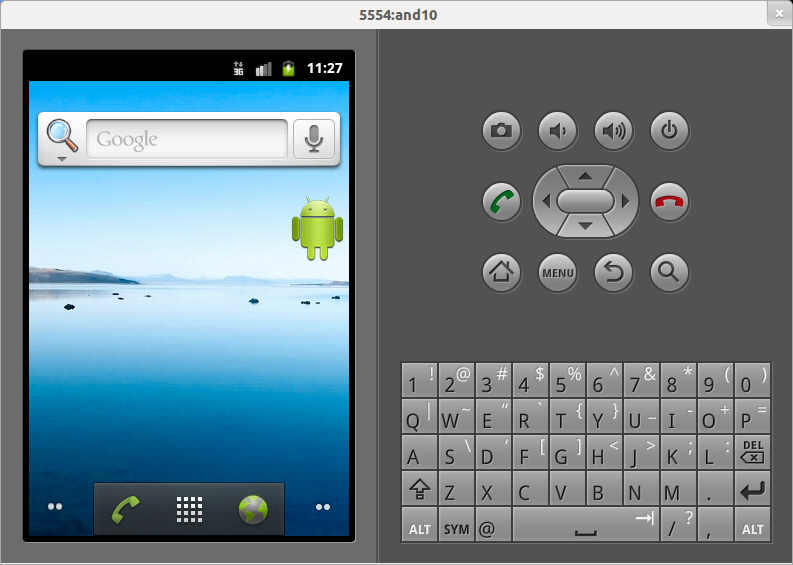
\includegraphics[width=14cm]{image/emulator.png}
  \caption{emulator模拟器}
\end{figure}

\lstinline!emulator!中模拟的Android系称为AVD(Android Virtual Device),由SDK中\lstinline!android!\cite{url:android_android}\index{android}工具创建:
\begin{lstlisting}[language=bash, numbers=none]
 $ android create avd -n my_avd -t android-10
\end{lstlisting}

可以使用图形化的AVD Manager直接启动AVD,也可以使用\lstinline!emulator!直接启动。使用命令行参数可以手工指定一些高级选项,这在一些分析时可能会用上。这些参数如下:
\begin{itemize}
\item \lstinline!-avd!,必选参数,指定AVD的名字
\item \lstinline!-data!,手工指定一个data分区镜像文件
\item \lstinline!-ramdisk!,手工指定一个RAM镜像文件
\item \lstinline!-kernel!,手工指定一个内核文件
\item \lstinline!-system!,手工指定一个system分区镜像文件
\item \lstinline!-sdcard!,手工指定一个SD卡镜像文件,该文件可以用\lstinline!mksdcard!创建
\item \lstinline!-dns-server!,给出DNS服务器地址,可以指向自己搭建的DNS服务器,模拟样本依赖的服务器
\item \lstinline!-http-proxy!,当样本访问被墙的网址时,可以通过SSH隧道和本地HTTP端口转发
\item \lstinline!-debug!,打开或关闭指定的调试标签,让\lstinline!emulator!输出调试信息,可以使用\lstinline!emulator -help-debug-tags!察看有哪些标签
\end{itemize}
例如,\lstinline!droidbox!的启动命令行是:
\begin{lstlisting}[language=bash, numbers=none]
 $ emulator -avd droidbox -system system.img -ramdisk ramdisk.img -kernel zImage -prop dalvik.vm.execution-mode=int:portable
\end{lstlisting}

\lstinline!emulator!的不足之处是:
\begin{itemize}
\item 虽然可以模拟短信和通话,但并没有与真正的移动通信网络相连
\item 对依赖于ROM环境、依赖于特定手机型号的样本不起作用
\end{itemize}

\subsection{手机}
手机可以提供运行样本的真实环境,并且与移动通信网相连。主要缺点是成本较高。

推荐Google的Nexus S型号手机,原因包括:
\begin{itemize}
  \item 直接使用Android源码可以编译Nexus S系统镜像,自行修改的源码可以获得真实的运行环境,并且可以对该镜像做自由的修改,比如有root权限、可以修改启动配置等
  \item 诸如TaintDroid、AppFence等项目均提供了用于Nexus S的源码
  \item 可以在第一时间获得新版本系统,例如Android 4.0
  \item 综合性价比较高
\end{itemize}

\subsection{Android-x86}
Android-x86\cite{url:android_x86}\index{Android-x86}提供了用于Intel x86处理器的Android系统镜像,可以将其安装到诸如VirtualBox和VMware WorkStation这样的虚拟机中。有研究称该项目系统的启动速度是\lstinline!emulator!中AVD启动速度的四分之一。

\section{设备管理}
\subsection{adb}
\lstinline!adb!是连接PC与设备(模拟器或手机)的主要工具,其用法在Android开发文档中有详细的说明\cite{url:android_adb}。

它的功能包括:
\begin{itemize}
\item 提供了一个访问Android底层Linux系统的shell
\item 通过push和pull在PC和设备之间传输文件
\item 通过install和uninstall安装或卸载应用程序
\item 转发对Android系统的调试指令和数据
\item 通过logcat获取系统进程和应用程序输出的日志信息
\end{itemize}

\subsubsection{shell}
输入下面的命令将连接设备并打开一个shell。
\begin{lstlisting}[numbers=none]
 $ adb shell
\end{lstlisting}
如果得到的提示符是\lstinline!\$!,是一个没有root权限的shell;如果提示符是\lstinline!\#!,则是有root权限的shell。

在设备系统的/system/bin目录下,提供了一些实用工具,例如Linux下常用的\lstinline!ls!、\lstinline!chmod!等,也有一些Android的小工具,例如\lstinline!am!等。

如果只是执行一两条指令,可以不进入交互式shell,而直接在本地完成,例如:
\begin{lstlisting}[numbers=none]
 $ adb shell ls /data/data
\end{lstlisting}

shell是在Linux层操作Android系统的主要方式。

\subsubsection{文件传输}
把本地文件发送至设备路径:
\begin{lstlisting}[numbers=none]
 $ adb push /path/to/local/file /path/to/device/target
\end{lstlisting}

从设备的指定路径获取文件:
\begin{lstlisting}[numbers=none]
 $ adb pull /path/to/device/file /path/to/local/target
\end{lstlisting}
这两条命令需要对设备端的路径和文件有相应的写和读的权限。如果权限不够,需要在root权限的shell下\lstinline!remount!分区;或者使用\lstinline!/data/local/tmp!目录作为中转站(普通权限的shell即可访问该目录),在root权限下做进一步拷贝。例如:
\begin{lstlisting}[numbers=none]
 host$ adb push ./tcpdump /data/local/tmp
 host$ adb shell
 device$ su
 device# cp /data/local/tmp/tcpdump /system/bin/tcpdump
 device# chmod 6755 /system/bin/tcpdump
 device# exit
 device$ exit
 host$
\end{lstlisting}

\subsubsection{安装和卸载}
将本地APK文件安装至设备很简单:
\begin{lstlisting}[numbers=none]
 $ adb install /path/to/local/app.apk
\end{lstlisting}

而与之相应的卸载则需要先知道应用程序的package name:
\begin{lstlisting}[language=bash, numbers=none]
 $ adb uninstall app.full.package.name
\end{lstlisting}
这个package name与该应用在设备系统的\lstinline!/data/data!路径下的子目录名完全相同。

\subsubsection{转发端口}
例如建立本地端口6100与设备端口7100之间的转发:
\begin{lstlisting}[numbers=none]
 $ adb forward tcp:6100 tcp:7100
\end{lstlisting}
这种转发将在后面的远程调试时使用。

\subsubsection{捕获日志}
使用:
\begin{lstlisting}[numbers=none]
 $ adb logcat
\end{lstlisting}
可以在本地终端显示应用程序的运行日志,例如调试信息和出错信息等。\lstinline!logcat!可以配合参数与日志过滤器,例如\lstinline!droidbox!的日志捕获使用的命令就是:
\begin{lstlisting}[numbers=none]
 $ adb logcat dalvikvm:W *:S
\end{lstlisting}
具体用法可以参考\lstinline!adb!的文档。

\subsection{ddms}
\begin{figure}[htbp]
  \centering
  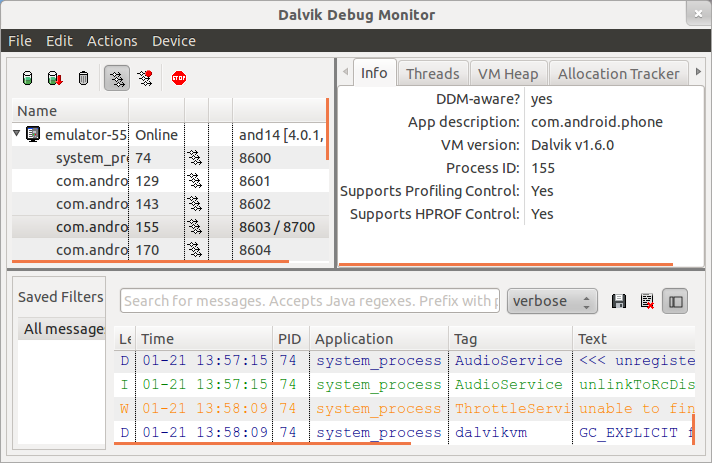
\includegraphics[width=14cm]{image/ddms.png}
  \caption{ddms的主界面}
\end{figure}
SDK中的\lstinline!ddms!\index{ddms}工具提供了一个可视化调试环境,功能包括:
\begin{itemize}
  \item 设备进程和线程管理
  \item 进程的内存管理
  \item 可视化logcat工具,以及图形化的过滤器
  \item 设备文件浏览
  \item 设备屏幕捕获
  \item dump设备状态和应用程序状态
\end{itemize}

\section{网络分析}
\subsection{tcpdump}
为了捕获样本在运行期间产生的网络数据,需要对其抓包。主要工具是\lstinline!tcpdump!\index{tcpdump}。针对不同的场景,可以在三个不同的位置使用这一工具。

\subsubsection{模拟器}
模拟器\lstinline!emulator!有一个没有公开的参数\lstinline!-tcpdump!,在启动模拟器时,通过该参数指定一个本地文件路径,可以将模拟器运行期间产生的所有网络数据捕获到指定的文件,该文件为PCAP格式,可以使用\lstinline!wireshark!或\lstinline!libpcap!解析。
\begin{lstlisting}[numbers=none]
 $ emulator -avd my_avd_name -tcpdump /path/to/dump.pcap
\end{lstlisting}
使用模拟器抓包的优点是不会捕获到本机其他进程产生的网络数据,缺点是:
\begin{itemize}
  \item 对真实手机显然无效
  \item Android系统在开机时大量使用网络端口传输调试信息等,因此捕获的PCAP数据包中有大量的无意义数据需要区分
\end{itemize}

\subsubsection{Android系统}
有移植到Android底层的原生\lstinline!tcpdump!工具,但其运行需要root权限。这一工具可以在模拟器中的系统里运行,但更多时候用于真实手机系统的抓包。
\begin{lstlisting}[numbers=none]
 host$ adb push ./tcpdump /data/local/tmp/tcpdump
 host$ adb shell
 device$ su
 device# chmod 6755 /data/local/tmp/tcpdump
 device# /data/local/tmp/tcpdump -p -vv -s 0 -w /sdcard/capture.pcap
\end{lstlisting}
其中,最后一行是启动\lstinline!tcpdump!,捕获一切数据包并保存在SD卡根目录下。不再需要捕包时,可以按下Ctrl + C终止。

在系统中使用原生\lstinline!tcpdump!的优点是能根据需要开始和结束捕包,并且在真实手机上也行之有效。主要缺点是要求拥有系统的root权限。

\subsubsection{Wi-Fi}
如果是没有root权限的手机,接下来的方法就只有通过Wi-Fi接入互联网,并且在网络上捕包了。例如,在无线路由器与网关之间加入一个集线器,在集线器上另外接一根网线到PC机上。由于集线器这种物理层设备会广播所有的网络流量,因此在PC上就可以捕获到手机通过无线路由器与Internet通信的所有数据。这种方案依然存在不足:
\begin{itemize}
  \item 会捕获到所有经过路由器的流量数据
  \item 极少数恶意代码只通过GPRS和3G联网
\end{itemize}

\subsection{Wireshark}
Wireshark\cite{url:wireshark}\index{Wireshark}是分析网络数据最常用也最强大的工具。在此不再专门介绍。

\section{行为模拟}
很多样本的恶意行为只在一定条件下触发,但在分析环境中,这些条件不一定能立即实现。此时需要对相应的条件进行模拟。在Android SDK文档中对此已经有一些介绍\cite{url:android_using_emulator}。

\subsection{am}
\lstinline!am!\index{am}是Android系统中的一个工具,位于/system/bin目录下,实际上是基于\lstinline!/system/framework/am.jar!执行\lstinline!com.android.commands.am.Am!类的代码。\lstinline!am!的主要作用即是启动活动(activity)、意图(intent)、广播(broadcast)等。

\lstinline!am!的用法如下:
\lstinputlisting[firstline=1, lastline=20, numbers=none]{code/am.txt}

其中,\lstinline!am start!用于启动一个活动;\lstinline!am startservice!用于启动一个服务;\lstinline!am broadcast!用于发送一个广播。它们的参数都是一个一个意图(Intent)。\lstinline!am!中intent的写法如下:
\lstinputlisting[firstline=76, lastline=101, numbers=none]{code/am.txt}

\subsection{telnet}

\subsection{DNS}

\subsection{openBTS}

\section{行为跟踪}
\subsection{droidbox}
\subsection{LBE}
\subsection{androidAuditTools}
androidAuditTools\cite{url:androidaudittools}

\section{调试}
\label{Sec:debug}
\subsection{apktool}
\subsection{AndBug}

\section{衍生文件}

%!TEX encoding = UTF-8 Unicode
\chapter{Dalvik虚拟机}
\label{Chap:dalvik}
Dalvik是专为Android设计的一种类JVM虚拟机,是Android应用程序的实际运行平台。从恶意代码分析的角度,Dalvik上DEX文件格式的重要性,相当于Windows上PE文件格式;Dalvik指令集的重要性,相当于PC上x86指令集的重要性。在静态分析中,分析人员有一半以上的时间是在与Dalvik指令打交道;在动态分析中,绝大部分时候没有恶意代码源码,也会涉及Dalvik级的调试;如果要将一些分析工作自动化,或展开一些研究,就不得不进行DEX格式的解析。

\section{Dalvik虚拟机的设计}
JVM是一个已经设计成熟并被实践检验过的成熟的虚拟机。但在Android这样的移动平台,存在CPU性能较低、可用内存极少、电力由电池供应、没有交换空间等限制,直接使用JVM运行复杂的应用程序较为困难。此外,使用JVM还存在许可的问题。因此,Dan Bornstein设计并实现了Dalvik虚拟(名字来源于冰岛的一个小渔村)。

从虚拟级别上来说,Dalvik是一个进程级的虚拟机,提供普通应用程序的运行环境,像Java语言的JVM、.NET平台的CLR一样。从体系结构来看,Dalvik是一个基于寄存器的虚拟机。

与JVM这种基于栈的虚拟机相比,基于寄存器的虚拟机在对相同应用程序的执行上快三分之一,还能从流水线型处理器获得额外的性能提升,并有更快的加载速度和更好的容错性\cite{dalvik_analysis}。

Dalvik运行于其底层的Linux进程中,执行DEX格式文件中的Dalvik指令。通过一些库(zlib、Java核心库、openssl等)实现功能和对系统的调用,通过JNI规范调用本地代码执行。Dalvik利用Linux进程的用户ID来管理文件访问权限,并实现内存隔离,通过Linux进程间通信在应用程序之间共享数据。
\section{DEX文件格式}
\subsection{类型描述符}
\label{SubSec:dalvik_data_type}
DEX格式中,使用缩略符号表示数据类型,如下表所示:

\begin{table}[htbp]
  \caption{Dalvik数据类型描述符}
  \label{Fig:dalvik_type}
  \centering
  \begin{tabular}{ll}
    \toprule
    \textbf{句法} & \textbf{含义} \\
    \midrule
    \lstinline!V! & \lstinline!void!,只能用于返回值 \\
    \lstinline!Z! & \lstinline!boolean! \\
    \lstinline!B! & \lstinline!byte! \\
    \lstinline!S! & \lstinline!short! \\
    \lstinline!C! & \lstinline!char! \\
    \lstinline!I! & \lstinline!int! \\
    \lstinline!J! & \lstinline!long! \\
    \lstinline!F! & \lstinline!float! \\
    \lstinline!D! & \lstinline!double! \\
    \lstinline!Lfully/qualified/Name;! & \lstinline!fully/qualified/Name!类 \\
    \lstinline![descriptor! & \lstinline!descriptor!类型的数组 \\
    \bottomrule
  \end{tabular}
\end{table}

例如,\lstinline![Ljava/lang/String;!表示\lstinline!String[]!。

\section{ODEX文件格式}
\label{Sec:odex}

\section{Dalvik指令集}
关于Dalvik指令集的主要参考文档是Android源码的dalvik/docs/dalvik-bytecode.html文件。本节的主要内容来自于该文档。

指令集的设计是一门艺术。从分析人员的角度考虑,不需要了解其中诸多细节。下面是指令集中为了便于人阅读的一些语法规则:
\begin{itemize}
  \item 两个操作数,前面是目的寄存器,后面是源寄存器
  \item 一般类型的64位opcode在32位opcode基础上加\lstinline!-wide!后缀;特殊类型opcode在一般类型opcode基础上加类型后缀,例如\lstinline!-char!、\lstinline!-int!、\lstinline!-long!、\lstinline!-float!、\lstinline!-string!、\lstinline!-object!等
  \item 对不是32位或64位操作的opcode,还加上特定后缀以说明其操作位数,例如\lstinline!/8!表示8位操作,\lstinline!/16!表示16位操作
\end{itemize}
例如,对指令\lstinline!move-wide/from16 vAA, vBBBB!,其中字段含义如下:
\begin{itemize}
  \item[move] 基本的opcode,说明指令功能
  \item[wide] 名称后缀,说明它操作64位数据
  \item[from16] 指令后缀,说明它的源操作数是一个16位寄存器
  \item[vAA] 目的寄存器,\lstinline!AA!是两个字母,表示寄存器的范围是\lstinline!v0!到\lstinline!v255!(一个字母表示4位)
  \item[vBBBB] 源寄存器,\lstinline!BBBB!是四个字母,表示寄存器的范围是\lstinline!v0!到\lstinline!v65535!
\end{itemize}
下面我们介绍Dalvik指令集,限于篇幅只列举和说明基本opcode,关于每个opcode可以适用的名称后缀、指令后缀、寄存器范围等,请参考dalvik/docs/dalvik-bytecode.html文件。
\begin{filecontents}{chapter-cn/LTXtable-dalvikopcode.tmp}
  \begin{longtable}{lX}
    \hline \textbf{基本指令} & \textbf{描述} \\
    \hline \lstinline!nop! & 空指令 \\
    \hline \lstinline!move! & 将源寄存器的值拷贝给目标寄存器 \\
    \hline \lstinline!move-result! & 将最近一次\lstinline!invoke!类型指令(函数调用)所返回的结果拷贝给指定的寄存器 \\
    \hline \lstinline!move-exception! & 将最近一次捕获到的异常值拷贝给指定寄存器 \\
    \hline \lstinline!return-void! & 在\lstinline!void!型的方法中返回,类似于C中的直接\lstinline!return! \\
    \hline \lstinline!return! & 在方法中,以指定寄存器的值返回 \\
    \hline \lstinline!const! & 将一个常量值(或常量字符串)赋给指定的寄存器 \\
    \hline \lstinline!monitor-enter! & 请求对指定目标的监视器 \\
    \hline \lstinline!monitor-exit! & 释放对指定目标的监视器 \\
    \hline \lstinline!check-cast! & 如果寄存器不能被动态转换为指定类型,就释放一个\lstinline!ClassCastException!异常 \\
    \hline \lstinline!instance-of! & 检查源寄存器中引用的值是否是指定类型数据,将结果1或0保存至目标寄存器 \\
    \hline \lstinline!array-length! & 将源寄存器指向的数组的长度取给目标寄存器 \\
    \hline \lstinline!new-instance! & 动态创建指定类型的一个新对象实例,将其引用值赋给目标寄存器 \\
    \hline \lstinline!new-array! & 动态创建指定类型的一个数组,其元素个数由源寄存器给出,将其引用值赋给目标寄存器 \\
    \hline \lstinline!filled-new-array! & 动态创建指定类型的一个数组,并以指定的值初始化,得到的结果必须使用\lstinline!move-result-object!来保存到特定寄存器,就像\lstinline!invoke!那样 \\
    \hline \lstinline!fill-array-data! & 以指定的数据填充一个数组 \\
    \hline \lstinline!throw! & 抛出一个指定的异常 \\
    \hline \lstinline!goto! & 无条件跳转至指定位置的指令 \\
    \hline \lstinline!packed-switch! & 测试寄存器的值,跳转到指定位置的指令\\
    \hline \lstinline!sparse-switch! & 测试寄存器的值,跳转到指定位置的指令,位置保存在排好序的值-偏移对中 \\
    \hline \lstinline!cmp! & 比较两个寄存器中的\lstinline!float!或\lstinline!double!或\lstinline!long!值,返回等于(0)、大于(-1)、小于(1)到目的寄存器 \\
    \hline \lstinline!if-!test & 例如\lstinline!if-eq!、\lstinline!if-lt!、\lstinline!if-ge!等,如果要比较的两个寄存器的值符合test条件,就跳转到指定偏移的指令 \\
    \hline \lstinline!if-!test\lstinline!z! & 与\lstinline!if-!test类似,但是是一个寄存器与0比较 \\
    \hline \lstinline!aget!,\lstinline!aput! & 根据索引读或者写一个数组(array)的指定元素 \\
    \hline \lstinline!iget!,\lstinline!iput! & 读或者写一个对象实例(instance)中的特定的域\\
    \hline \lstinline!sget!,\lstinline!sput! & 读或者写一个静态域(static field)中的特定的域\\
    \hline \lstinline!invoke-!kind & 函数调用,类型kind包括:\lstinline!virtual!虚方法、\lstinline!super!最近的父类的虚方法、\lstinline!direct!非静态直接方法、\lstinline!static!静态方法、\lstinline!interface!接口方法\\
    \hline unop & 单变量算术运算,例如\lstinline!neg-int!取整数的补码、\lstinline!long-to-float!将长整数转换为浮点数等等 \\
    \hline binop & 双变量算术运算,例如\lstinline!sub-int!整数相减,\lstinline!shr-long!长整数算术右移等等 \\
    \hline 
  \end{longtable}
\end{filecontents}
\LTXtable{\textwidth}{chapter-cn/LTXtable-dalvikopcode.tmp}

\section{smali语法}
由于在静态分析时smali反汇编得到Dalvik指令是目前最常用的一种方法,本节基于smali的语法对Dalvik指令集做进一步介绍。

本节的代码来自于lohan+在其博客\footnote{\url{http://androidcracking.blogspot.com},这个关于Android逆向和破解技术的博客上有很多不错的文章,建议仔细阅读}上发表的两篇相关教程,他已经授权本文使用,在此表示感谢。

其中涉及大量关于Dalvik中数据类型的语法,请回顾第\ref{SubSec:dalvik_data_type}节。

\subsection{smali源文件}
先来看一个smali源文件,比较长,我们在后面逐一解释:
\lstinputlisting[language=smali, caption={smali源文件示例}]{code/example.smali}

第1行指明该文件所定义的类的名称\lstinline!com.packageName.example!,以及类属性\lstinline!public!;第2行指明该类的父类为\lstinline!java.lang.Object!;第3行指明该文件的文件名为example.java:
\lstinputlisting[language=smali, firstline=1, lastline=3, firstnumber=1]{code/example.smali}

第5和7行给出了类的两个域实例,一个是名为someInt的整型变量,一个是名为someBool的布尔型变量:
\lstinputlisting[language=smali, firstline=5, lastline=7, firstnumber=5]{code/example.smali}

接下来是该类的构造函数。先看一下这个函数的开始几行:
\lstinputlisting[language=smali, firstline=9, lastline=14, firstnumber=9]{code/example.smali}
第9行的\lstinline!.method!前缀说明下面是一个函数,\lstinline!public!说明其作用域,\lstinline!constructor!说明其是类的构造函数,使用了默认的\lstinline!<init>!作为供人阅读的函数名(显然,构造函数的真实函数名与类名相同)。接下来的\lstinline!(ZLjava/lang/String;I)V!需要注意,其中括号内是参数类型列表,多个参数直接写在一起,不使用任何符号分隔,括号后是返回值类型。在这个构造函数中,有三个参数,第一个参数\lstinline!Z!是布尔型;第二个参数\lstinline!Ljava/lang/String;!是Java中的字符(注意在以\lstinline!L!开头接对象全称的这种参数语法上,最后以分号结尾以划分与后面类型的界限);第三个参数\lstinline!I!是整型。返回值是\lstinline!V!,即\lstinline!void!型。因此,这个构造函数的原型为:
\begin{lstlisting}[language=java, numbers=none]
public void example(boolean someBool, String exampleString, int someInt);
\end{lstlisting}
如果对这一部分还不理解,请回过头再看一下\ref{SubSec:dalvik_data_type}一节。

第10行指出这个函数需要使用六个寄存器来存储局部变量,在函数内部分别记为\lstinline!v0!、\lstinline!v1!到\lstinline!v5!。

第12到14行给出了三个参数的名称。注意有时候代码被混淆后,这部分信息将丢失。另外注意这里列举的顺序与函数实际参数顺序并不一致。

\lstinputlisting[language=smali, firstline=16, lastline=18, firstnumber=16]{code/example.smali}
第16行的\lstinline!.prologue!可以直接忽略。第17行的\lstinline!.line 10!标明行号,主要在调试时使用。

第18行出现了函数调用\lstinline!invode-direct!。其中,\lstinline!p0!是指参数0,即\lstinline!this!指针,这条语句调用了父类\lstinline!java.lang.Object!的构造函数,其参数为空,返回值为\lstinline!void!。

\lstinputlisting[language=smali, firstline=20, lastline=26, firstnumber=20]{code/example.smali}
第20行,将一个字符串的引用值赋给了局部寄存器\lstinline!v0!;第22行,将常量0xf(也就是十进制的15)赋给局部寄存器\lstinline!v0!,这会导致之前保存的字符串引用值丢失。

第24到26行,动态分配了一个\lstinline!java.lang.StringBuilder!对象,将其引用值赋给\lstinline!v1!,又将一个字符串的引用值赋给\lstinline!v2!,最后调用了\lstinline!v1!指向的\lstinline!StringBuilder!对象的构造函数,将\lstinline!v2!作为参数。注意第26行的\lstinline!invoke-direct!指令,其后的\lstinline!{v1, v2}!,第一个参数和第二个参数的不同作用。

\lstinputlisting[language=smali, firstline=28, lastline=29, firstnumber=28]{code/example.smali}
第28行,调用了\lstinline!v1!指向\lstinline!StringBuilder!对象的\lstinline!append(boolean)!方法,其参数使用\lstinline!p1!,即该函数的第一个实际参数\lstinline!boolean someBool!。注意这条指令的返回值是一个新的\lstinline!java.lang.StringBuilder!对象,在第29行,将这个返回值重新赋给了\lstinline!v1!。综上,第20到29行的源码应该是:

\begin{lstlisting}[language=java, numbers=none]
  StringBuilder a = new StringBuilder("the spice must flow");
  a = a.append(someBool);
\end{lstlisting}

我们跳过几行,直接看到第38行:

\lstinputlisting[language=smali, firstline=38, lastline=40, firstnumber=38]{code/example.smali}
可以看到,在39行,调用了\lstinline!android.util.Log!中的\lstinline!int d(String, String)!这个静态方法,注意这里使用了恰当的\lstinline!invoke-static!指令,并且其两个参数\lstinline!{v0, v1}!直接作为了\lstinline!d()!的两个参数,而不再像前面\lstinline!invoke-direct!那样第一个参数是方法所在对象的句柄。

再来看第50行:
\lstinputlisting[language=smali, firstline=50, lastline=50, firstnumber=50]{code/example.smali}
使用了\lstinline!iput-boolean!指令,前面已经介绍,\lstinline!iput!是对对象实例中域的操作,这里对象实例由\lstinline!p0!给出,取出其名为\lstinline!someBool!的域,赋给\lstinline!p1!。注意这里遇到了一个名称作用域的问题,当前函数的第一个参数叫\lstinline!someBool!,当前类实例有一个域也叫\lstinline!someBool!,由于使用的\lstinline!iput!,因此这里使用类实例的域。这一行代码等价于源码:
\begin{lstlisting}[language=java, numbers=none]
  someBool = this.someBool;
\end{lstlisting}

最后,在第61行,这个构造函数使用\lstinline!return-void!指令退出。到此,读者可以尝试自己阅读和分析第64到78行的\lstinline!someMethod!方法。

\subsection{常用代码结构}
无论是学习哪个指令集的反汇编,最好的方法都是自己动手将常见的代码结构写出来、编译好,再反汇编,将源码与反汇编结果对应起来看。lohan+再次为我们提供了这样的资源。

\subsubsection{构造函数和域}
\lstinputlisting[language=java, firstline=8, lastline=11, firstnumber=8, caption={构造函数、域的Java示例}]{code/example-structures.java}
\lstinputlisting[language=smali, firstline=5, lastline=18, firstnumber=5, caption={构造函数、域的smali示例}]{code/example-structures.smali}

Java中的静态变量,也就是域\lstinline!Count!,在smali中被\lstinline!.field!引导申明,说明其是一个静态私有\lstinline!int!型变量。

Java中类\lstinline!example!的构造函数,在smali中被\lstinline!.method!引导并被\lstinline!constructor!修饰,其方法名变成了\lstinline!<init>!。注意在第12行,该方法显式地调用了其父类的构造函数(同样以\lstinline!<init>!命名)。

在代码的第15行,\lstinline!sput!指令的作用是赋给一个域变量指定的值。注意域是类有关而与具体对象无关的,因此需要使用\lstinline!Lcom/lohan/crackme1/example;!来指出其归属关系。这也是为什么\lstinline!sput!需要单独作为一条指令。

\subsubsection{for结构}
\lstinputlisting[language=java, firstline=13, lastline=17, firstnumber=13, caption={for结构的Java示例}]{code/example-structures.java}

\lstinputlisting[language=smali, firstline=62, lastline=97, firstnumber=62, caption={for结构的smali示例}]{code/example-structures.smali}

首先注意第70行和79行有两个标签\lstinline!:goto_1!和\lstinline!:cond_6!,这种标签用于标记代码位置,用于\lstinline!goto!跳转。

接下来看代码。在67行,定义了一个局部整形变量(在69行给出其名字信息\lstinline!i!),初始化为\lstinline!0!。在71行,将\lstinline!com.lohan.crackme1.example!类的域\lstinline!Counter!的值取到寄存器\lstinline!v1!。

然后在73行将\lstinline!i!与\lstinline!v1!作比较,使用的是\lstinline!if-lt!指令。注意这条指令的第三个操作数为标签\lstinline!:cond_6!。这条指令的执行效果是:如果\lstinline!i!比\lstinline!v1!小(less-than),就跳转到\lstinline!:cond_6!标记的位置;否则顺序执行,即执行\lstinline!return-void!返回。

当跳转到\lstinline!:cond_6!后,我们来看第80行到91行,它们对应的Java源码只有一行:
\begin{lstlisting}[language=java, numbers=none]
System.out.println("current val for loop: " + i);
\end{lstlisting}
但在smali中,使用了四个\lstinline!invoke!才完成。主要流程是:取\lstinline!java.lang.System!类的\lstinline!out!域,它是一个\lstinline!java.io.PrintStream!对象;创建一个\lstinline!java.lang.StringBuilder!对象;用固定的字符串初始化这个对象;用该对象的\lstinline!append!方法将\lstinline!i!加到字符串后面;用该对象的\lstinline!toString!方法转化为字符串对象;最后,调用\lstinline!out!的\lstinline!println!方法,打印出这个字符串。

由此可以看出,smali代码实际上已经到了Java VM opcode的细致程度,要精通smali,对JVM指令集的了解是需要的。

最后,在打印完字符串以后,在94行,通过\lstinline!add-int!指令,让\lstinline!i!加\lstinline!1!,然后跳转到\lstinline!:goto_1!的位置继续执行下一次循环。

这就是smali中\lstinline!for!循环的标准结构:两个位置标签,一个用于没有越界时跳过\lstinline!return!语句,一个用于加1后循环。

\subsubsection{switch结构}
\lstinputlisting[language=java, firstline=19, lastline=29, firstnumber=19]{code/example-structures.java}
\lstinputlisting[language=smali, firstline=99, lastline=158, firstnumber=99]{code/example-structures.smali}

\subsubsection{try-cache结构}
\lstinputlisting[language=java, firstline=31, lastline=46, firstnumber=31]{code/example-structures.java}
\lstinputlisting[language=smali, firstline=160, lastline=262, firstnumber=160]{code/example-structures.smali}

\subsubsection{数组}
\lstinputlisting[language=java, firstline=48, lastline=59, firstnumber=48]{code/example-structures.java}
\lstinputlisting[language=smali, firstline=20, lastline=60, firstnumber=20]{code/example-structures.smali}


%!TEX encoding = UTF-8 Unicode
\chapter{ARM漏洞利用}
\section{学习的目的}
目前,绝大部分智能移动终端使用ARM处理器,包括基于Android、iOS、Symbian、Windows Mobile、Windows Phone等操作系统的手机和平板电脑。ARM还被大量的嵌入式设备使用。

使用ARM处理器的PC也已经出现。几年前,Debian就发布了ARM移植版;2011年,Ubuntu开始支持ARM;2012年将正式发布的Windows 8也已经被微软移植到ARM上。预计在2012年,使用ARM处理器的笔记本电脑将开始流行。

ARM还开始向服务器市场发展。目前,Nvidia和巴塞罗那超级计算中心还推出了基于ARM和CUDA计算的超级计算机,Nvidia也将在2012年初向普通开发者推出基于ARM的CUDA开发工具。

可以看出,ARM设备无论是数量上还是覆盖面都不逊色于PC。但ARM的安全问题,尤其是其上软件漏洞的问题,直到近几年才引起人们的注意。
\section{环境和工具}
\subsection{ARM设备和系统}
\subsubsection{开发板}
获得一个ARM设备的常规方法是购买或者定制ARM开发板。如果不打算移植Android等系统,可以选择mini2440,否则可以选择mini6410等型号。

需要自己为开发板交叉编译操作系统,并烧录进去。这个过程会比较好玩。但如果觉得乏味,或者时间不够,可以使用Ångström发行版\footnote{\href{http://www.angstrom-distribution.org/}{http://www.angstrom-distribution.org/}}。

开发板的优点是,它是一个真实的ARM设备和运行环境;缺点是操作稍显繁琐。除此以外,还有其他方法可以获得ARM系统。

\subsubsection{Android模拟器或手机}
Android手机本身就是一个ARM设备,而Android底层的Linux内核就是运行于ARM上的系统。因此,Android手机基本是可以充当ARM开发和调试环境的。此外,Android SDK中的模拟器也是基于qemu模拟了ARM设备。从漏洞分析和漏洞利用的角度来看,使用Android手机或模拟器进行学习的优点包括:

\begin{itemize}
\item 如果要分析Android的漏洞,这自然是最佳的选择
\item 有完善的开发工具链和系统源码
\item 模拟器的硬件(边际)成本为0
\end{itemize}

但缺点也不少:

\begin{itemize}
\item 在Android中的Linux上,没有太多的本地应用程序,例如gdb等调试工具(只有gdbserver)
\item 不使用glibc库,而是自行开发的bionic,因此一些利用技巧在细节上会和Linux(on ARM)有差异
\item 目标文件的编译,或者完全静态链接,或者用NDK开发,或者与Android源码一起编译,均显繁琐
\end{itemize}

无论如何,模拟器完全没有成本,建议在PC中常备以便使用。

\subsubsection{Debian虚拟机}
早在2000年,Debian就开始了对ARM处理器的移植工程,目前其仓库中几乎所有的软件都有了ARM版本,包括objdump、gdb等常用开发和漏洞分析工具。

另一方面,qemu模拟器已经可以完美地模拟ARM处理器及其硬件平台,可以用它在x86的PC上运行ARM版的Debian。

可以直接从Debian的官网下载到其ARM安装包,然后参考aurel提供的安装指南\footnote{\href{http://www.aurel32.net/info/debian\_arm\_qemu.php}{http://www.aurel32.net/info/debian\_arm\_qemu.php}}。

更省事的方案是直接下载已经安装好的qemu镜像,也是由aurel提供。包括arm版\footnote{\href{http://people.debian.org/~aurel32/qemu/arm/}{http://people.debian.org/$\sim$aurel32/qemu/arm/}}
和armel版\footnote{\href{http://people.debian.org/~aurel32/qemu/armel/}{http://people.debian.org/$\sim$aurel32/qemu/armel/}}
,建议使用后者。

\subsubsection{Toshiba AC100}
Toshiba AC100是目前唯一一款拥有标准全键盘的ARM笔记本。它最初是为Android设计,但hackers已经将多个Ubuntu版本移植到该机器上。最终,Canonical公司从Ubuntu 11.10开始专门为这一机器提供预编译版本和软件源,作为其向ARM平台扩张的第一步。

该机器在国内的型号为AC100-01B,已经不再生产,但可以购买到二手的。

这个笔记本是目前唯一一种可以最轻松获得的真实ARM机器,并拥有前面提到的Debian虚拟机的一切优点。

此外,在前面所述的方案中,除了4.0以上Android,其Linux Kernel均未开启ASLR(地址空间布局随机化)特性,但在Ubuntu for AC100中,开启了ASLR。这固然为简单的ret2libc等攻击带来了困难,但另一方面,也成为几乎是唯一的分析ASLR下漏洞的环境。考虑到Android 4.0开始去掉prelink优化、全面开启ASLR特性\cite{aslr_android},这种研究的价值是显然的。

\subsubsection{Nokia N900手机}
另一个hack利器是Nokia N900手机,这款老手机采用已经被抛弃的Maemo系统,该系统是基于Linux的手机操作系统,开放性较高。N900的键盘操作性不强,系统也适合于有hack精神的人玩。
\subsection{交叉编译工具}
进行嵌入式开发时,编译工具运行于一个平台,但生成另一个平台的指令,这种编译过程称之为交叉编译,所使用的编译工具又称之为工具链。

在x86上编译ARM代码最常用的工具链由CodeSourcery公司免费提供,有Windows版本和Linux版本\footnote{\href{http://www.mentor.com/embedded-software/sourcery-tools/sourcery-codebench/editions/lite-edition}{http://www.mentor.com/embedded-software/sourcery-tools/sourcery-codebench/editions/lite-edition}}。

此外,在基于Debian的系统(例如Ubuntu)中,也可以通过\lstinline!apt-get install gcc-arm-linux-gnueabi!直接获得一个交叉编译gcc。

Android的NDK中实际上也包含了完整的工具链,包括编译器、调试器、binutils等。它同样有Windows和Linux版本\footnote{\href{http://developer.android.com/sdk/ndk/index.html}{http://developer.android.com/sdk/ndk/index.html}}。

然而NDK也有不足,即只能为Android编译代码,也只能使用其提供的有限的库接口。对后面一个问题,如果需要编译使用了Andrid系统中较底层API的ARM程序,建议使用agcc工具,具体可以看我写的文章\footnote{\href{http://blog.claudxiao.net/2011/10/android_agcc/}{http://blog.claudxiao.net/2011/10/android\_agcc/}}。
\subsection{反汇编和反编译工具}
工具链包含了很多的工具,如果静态反汇编,可以使用\lstinline!objdump!;如果动态运行起来,在\lstinline!gdb!中也可以使用\lstinline!disass!反汇编。

对ARM反汇编支持最好的工具是IDA Pro,但它是商业软件。自由开源的反编译工具可以考虑radare\footnote{\href{http://www.radare.org/y/}{http://www.radare.org/y/}}或者smiasm\footnote{\href{http://code.google.com/p/smiasm/}{http://code.google.com/p/smiasm/}},但radare和smiasm对Thumb、Thumb-2指令集的支持都不强。

对这三个工具在ARM反汇编上的对比可以参考我的文章\footnote{\href{http://blog.claudxiao.net/2011/12/arm-disassemblers}{http://blog.claudxiao.net/2011/12/arm-disassemblers}}。

事实上,ARM的指令编码并不复杂,自己写一个ARM反汇编器的工作量远小于想象。

目前ARM的反编译工具只有Hex-Rays ARM Decompiler,是一款昂贵的收费软件。
\subsection{远程调试}
可以使用\lstinline!gdb!远程调试ARM设备或虚拟机中的程序。假设设备的IP地址是192.168.0.2,要调试的程序名为demo,则在设备端运行:
\begin{lstlisting}[language=bash, numbers=none]
  $ gdbserver 192.168.0.2:23456 /path/to/demo
\end{lstlisting}

接下来,在主机端使用ARM工具链中的gdb调试:
\begin{lstlisting}[language=bash, numbers=none]
  $ arm-eabi-gdb /path/to/demo
\end{lstlisting}

在进去gdb调试会话后,键入:
\begin{lstlisting}[language=bash, numbers=none]
  (gdb) target remote 192.168.0.2:23456
\end{lstlisting}

即可开始调试。

也可以使用IDA Pro远程调试Android系统,Berry写过一篇文章介绍操作方法\footnote{\href{http://debugman.com/thread/6230/1/1}{http://debugman.com/thread/6230/1/1}}。
\section{ARM体系结构}
\subsection{ARM指令集}
ARM同时是三个不同事物的名字:
\begin{itemize}
\item 一个公司
\item 一种体系结构
\item 一系列CPU产品
\end{itemize}
这一章主要是指第二种含义。

ARM是32位RISC结构,在ARMv5以后,基本采用Harvard结构,与传统的冯诺依曼结构不同的是,数据和代码被最大程度隔离了。既便于数据段保护的x86也有本质区别,ARM的代码和数据采用不同的总线传输(并因此获得并行而提速)。其数据段自然不能被执行。

\subsubsection{寄存器}
对程序员可见的寄存器主要是r0到r15共16个,不同的寄存器有不同的用途,将在下一节说明。

此外,有程序状态寄存器PSR,其中包括算数逻辑运算标志、执行状态位、当前中断号等。

\subsubsection{数据操作指令}
基本形式是:
\begin{lstlisting}[numbers=none]
<opcode>{<cond>}{S} <Rd>, <Rn>{, <operand2>}
\end{lstlisting}
其中:
\begin{itemize}
\item[opcode] 比如MOV、ADD,与x86类似,具体可以查ARM手册
\item[cond] 可选的条件码。条件执行是ARM的特色之一,几乎所有的ARM指令都可以加上条件码,实现条件执行。例如,EQ、LE等
\item[S] 可选的S位,如果该条指令会更改PSR,则应置上S位
\item[operand] 操作数可以是寄存器,也可以是一个右值(后面会说明),每条指令有多少操作数,分别是什么含义,应查手册
\end{itemize}

ARM中的右值操作数可以是一个寄存器、一个立即数,或者一个寄存器的移位。例如,右值R1, LSL \#2由R2的值逻辑左移2位得到,右值R1, ASR R3由R1的值算术右移R3位得到。

\subsubsection{分支跳转指令}
\begin{itemize}
\item[B] 直接跳转到一个地址,唯一的参数是12位立即数,与x86中的jmp功能一样
\item[BL] 将下一条指令地址(即返回地址)赋给LR寄存器,然后跳转到参数指定的地址,参数是一个12位立即数。BL与x86中的call功能一样
\item[BX] 参数是一个寄存器,跳转到该寄存器指向的地址
\end{itemize}
所有这些分支跳转指令都可以使用条件码,成为相应的条件跳转指令。

\subsubsection{内存访问指令1}
ARM使用简单的访存模型,所有内存读写都通过LDR和STR两条指令完成,而且只能在寄存器与内存之间读写,不能直接从内存读写到内存。LDR和STR都有一个可选的后缀B,不选时按字(4字节)读写,选择B时按字节读写。其第一个参数是寄存器,第二个参数是内存地址。

\subsubsection{寻址方式}
第一类寻址方式:
\begin{itemize}
\item 寄存器加上立即数偏移:[reg, \#$\pm$imm12]
\item 寄存器加上寄存器偏移:[reg, $\pm$reg]
\item 寄存器a加上移位后的寄存器b偏移:[rega, $\pm$regb, shift]
\end{itemize}
这些地址符号后面可以选择一个叹号:!。如果加上,表明先根据寻址规则修改寄存器,然后根据寄存器中的值访问内存;如果不加叹号,表示直接根据寻址规则访问内存。

第二类寻址方式则是先根据寄存器中的值访问内存,然后按照相应的规则更新寄存器:
\begin{itemize}
\item 访存后,寄存器加上立即数:[reg], \#$\pm$imm12
\item 访存后,寄存器加上寄存器:[reg], $\pm$reg
\item 访存后,寄存器a加上移位后的寄存器b:[rega], $\pm$regb, shift
\end{itemize}

\subsubsection{内存访问指令2}
还可以一次性读写多个字:
\begin{lstlisting}[numbers=none]
LDMcdum reg!, mreg
STMcdum reg!, mreg
\end{lstlisting}
其中:
\begin{itemize}
\item[cd] 可选的条件
\item[um] 访问模式,分别为IA读写后增加寄存器值、DA读写后减少寄存器值、IB读写前增加寄存器值、DB读写后增加寄存器值
\item[!] 表示会修改寄存器,修改方法参考um
\item[mreg] 支持一次指令多个寄存器,例如{R0-R3, R7, R10}
\end{itemize}

\subsection{ATPCS}
\subsubsection{名词解释}
例程(routine)、子例程(subroutine):对于一段可以调用、可以返回、保证栈平衡的代码片段,例程指调用者,子例程指被调用者。

过程(procedure):不返回结果值的例程。

函数(function):返回结果值的例程。

变量大小、内存对齐、字节序、复合类型等略。
\subsubsection{寄存器的用途}

ARM中有16个通用寄存器r0 – r15。其中:
\begin{itemize}
\item[r0 – r3] 用于传递参数、返回函数结果,因此又名a0 – a3。在例程内部也被用于保存临时结果
\item[r4 – r11] 用于保存例程内的局部变量值,又名v0 – v8。其中,r9(v6)是一个平台相关的值,不同的ARM平台必须为这个寄存器赋予特殊的含义
\item[r12 – r15] 有专门的用途,后面介绍。常用别名:IP、SP、LR、PC
\end{itemize}
\subsubsection{栈结构}

r13(SP)是栈指针。ARM中使用向下的满栈(full-descending),即SP始终指向最后一个已进入栈的数据,每次压栈时,SP自减需要的内存大小,然后将值存到SP新的位置。

也就是说,对栈的push相当于STMDB,对栈的pop相当于LDMIA,但一般不用这个后缀,而用STMFD和LDMFD。

SP的值应在栈的有效区间内,且mod 4 = 0。栈上有例程的调用帧结构。不要轻易地修改这个值。

\subsubsection{子例程调用}

ARM和Thumb指令集均有一个BL指令,它的操作是:将BL指令顺序下一条指令的地址(即返回地址)送入链接寄存器LR(r14),然后将调用的目的地址(即子例程地址)送入寄存器PC(r15)。

如果在Thumb中调用BL,则LR的第0位被设为1,否则被设为0。(因为指令地址要4字节对齐,因此LR的第0和1位都没有用。)

子例程返回很简单,将LR的值送入PC即可。

任何模拟上述过程的指令序列也会起到BL的效果,例如:mov LR, PC; BX r4。注意,任何时候读PC,得到的值是当前指令地址+8(why?请自己google)。

\subsubsection{结果返回}
\begin{itemize}
\item 不超过4字节的结果,一律用r0返回
\item 超过4字节的基本类型,继续用r1, r2, r3
\item 超过4字节的复合类型,或动态大小的结果,存储在内存中,并将其地址作为调用参数之一传入
\end{itemize}
\subsubsection{参数传递}

使用r0 – r3传递参数,如果不够,使用栈。

语言中的数据类型会按照相关标准转化为机器数据类型。
\section{ARM漏洞利用的特点}
与x86相比,ARM下要做到漏洞利用存在以下问题:
\begin{itemize}
\item 从v5开始,ARM普遍采用哈佛结构,数据段不可执行
\item 函数调用时,参数传递不再通过栈,而是使用寄存器
\item 返回地址按照ATPCS是通过LR寄存器传递,大部分被掉用函数会在其代码开始时将LR再次保存到栈上,在返回前从栈中直接取回至PC寄存器
\item 由于体系结构的本质区别,作为跳板的指令无法使用x86下常见的那些,而要根据实际需要来寻找
\end{itemize}
但也有好的消息。在Windows/x86平台引入DEP以后,因为代码部分的不可执行,出现的ret2libc和ROP等技巧,其思路也可以用于ARM。此外,ARM单条指令的描述能力是超过x86的,所以要寻找到合适的跳板指令序列并不是太难。

ARM漏洞利用是一个新的领域,目前参考文献较少,主要有\cite{arm_exploiting_linux}、\cite{arm_stack_exploitation}、\cite{arm_exploitation}、\cite{arm_ropmap}和\cite{arm_alphanumeric}。
\section{简单的示例}
\subsection{源代码}
下面我们看一个实际的例子。这个程序来自于\cite{arm_exploiting_linux},但因为编译源码使用的系统和编译器不同,后面的细节与原文有较大差异。
\lstinputlisting[language=c,caption={存在漏洞的示例代码}]{code/arm.test.c}

\subsection{反汇编结果}
如果使用的Toshiba AC100做实验,在Ubuntu下,从6.10开始gcc默认开启了-fstack-protector开关,存在不安全拷贝函数调用的函数,在退出前会做栈有效性检测(\_\_stack\_chk\_fail),因此进一步的漏洞利用会失败。应该在gcc编译时使用-fno-stack-protector来关闭这个开关。此外,在Toshiba AC100中,gcc默认将目标代码优化为Thumb指令集。后面的分析是基于ARM指令集的。可以给gcc加上-marm开关来强制指定其编译为ARM指令集。最后,也就是说,在AC100下,应该这样编译:

\begin{lstlisting}[language=bash, numbers=none]
  $ gcc test.c -o test -marm -fno-stack-protector
\end{lstlisting}

在编译完成后,就可以使用gdb来反汇编vuln()函数了。下面是在ARMEL的Debian系统下,用gcc4.4编译的结果:

\lstinputlisting[caption={vuln函数的反汇编结果}]{code/arm.test.dis1.asm}

逐一解析这些代码,以熟悉ARM指令。

在第3行,先后push了r11和lr寄存器。r11又称fp(帧指针寄存器),相当于x86下的ebp寄存器。它在该函数中使用了,所以将原来的值保存在栈中。lr前面有介绍,在调用该函数时将返回地址保存在了其中,因为在vuln()中还要bl到strcpy,还要用到lr,所以将lr保存在栈中,直到函数返回时(13行),才从栈中取出。这一点需要额外说明,虽然ATPCS规定由lr保存返回地址,且各编译器也遵循了这一约定,但在实现中,由于存在漏洞的函数其内部必然调用了其他函数,因此lr一定会在该函数的初始化时被保存到栈上,因此溢出是一定可以覆盖到它的。也就是说,虽然ATPCS的返回方法和x86的约定不同,但实际情况还是差不多。

第4行,给r11(fp)赋值。再次强调,ARM使用向下递减的满栈,因此r11指向sp加4,即栈顶第二个元素的地址。

第5行,sp自减24,开出了24字节的局部变量缓冲区。注意这里的\#24的立即数表示是十进制,而不是十六进制。

第6、7、10行,r0传给r3,r3传给r1。回忆ATPCS,r0中存着vuln()函数的第一个参数,即char *arg的值。调用strcpy时,r1是第二个参数,因此,将arg作为了strcpy的第二个参数。

第8、9行,在局部变量缓冲区取了12个字节的缓冲,给r0,作为strcpy的第一个参数。有人会奇怪,在源码中我们为buff申请了10个字节的缓冲,为什么这里成了12。这是因为ARM的内存访问都是4字节对齐的。

第11行,调用了strcpy函数。

第12行,恢复栈指针。

第13、14行,恢复r11原来的值,恢复lr的值,跳转至lr以返回。但很多编译器不这么实现,而是直接pop \{r11, pc\}。

可以看到,如果在strcpy时,输入的数据超过12个字节,就会逐步覆盖栈中保存的原来的r11(超过4字节)和lr(再超过4字节)。而lr会在后面取出作为函数返回地址。这样,就有可能通过覆盖栈来改变指令执行流程。

\subsection{栈结构}
我们再来看看当正常运行到上面第12行,即执行完strcpy后,栈的情况。我们用1234作为参数。

\lstinputlisting[caption={正常拷贝后的栈结构}]{code/arm.test.dis2.asm}

可以看到,参数1234已经出现在栈上(0xbedb9794处),而返回地址位于0xbedb97a4处,为0x0084ac。如果输入数据越界,则其17到20字节将正好覆盖这一返回地址。这个结论与我们前面对代码的分析是一致的。

\subsection{构造溢出}
从上面的栈结构,我们可以构造溢出数据了。如下所示:

\lstinputlisting[caption={构造溢出数据}]{code/arm.test.dis3.asm}

我们先看下donuts()函数的地址,为0x00008438,再考虑不破坏其他栈结构,因此构造了长为20字节的输入数据。其前12个字节随便填充,13-16字节为原来栈上的r11值,17-20字节为我们想要的返回地址,即donuts()函数的地址。最后,可以看到donuts()函数确实运行了起来,程序也正常退出了。

\section{漏洞攻击方法}
上述示例只是一个演示性的栈溢出。如果要发起真实攻击,跳到一个本地函数并不是我们需要的。

在x86中,最初的做法是将shellcode作为数据传给程序,程序将其放在溢出后的栈上。当函数退出时,跳转到栈上执行shellcode。在引入DEP后,栈上数据不可执行,从而产生了包括ret2libc在内的ROP技术,即跳转到一些系统API或库函数,通过控制这些API的参数实现一定的能力。

在x86上,参数是通过栈传递的。也就是说,通过栈溢出几乎一定可以把参数安置好,并调用其他函数。但在ARM上这一招没法直接用了。ATPCS规定使用r0 - r3这四个寄存器传递参数,而通常栈溢出是无法影响到这些寄存器的。只能寄希望于在溢出后,存在这类指令序列:将栈上的值拷贝至r0 - r3中。

以此思想为基础,Avraham提出了所谓的Ret2ZP(Return to Zero Protection)的攻击方法,主要在\cite{arm_stack_exploitation}和\cite{arm_exploitation}中进行了阐述。

\section{zergRush分析}
\subsection{背景和原理}
Revolutionary工具开发小组在2011年10月发布了一个在Android 2.2和2.3上获得root权限的方法\footnote{\href{http://forum.xda-developers.com/showthread.php?t=1296916}{http://forum.xda-developers.com/showthread.php?t=1296916}},并公布了漏洞利用代码zergRush.c\footnote{\href{https://github.com/revolutionary/zergRush/blob/master/zergRush.c}{https://github.com/revolutionary/zergRush/blob/master/zergRush.c}}。tomken\_zhang已经在其博客上发表了两篇文章对其分析\footnote{\href{http://blog.csdn.net/tomken\_zhang/article/details/6866260}{http://blog.csdn.net/tomken\_zhang/article/details/6866260}\newline\href{http://blog.csdn.net/tomken\_zhang/article/details/6870104}{http://blog.csdn.net/tomken\_zhang/article/details/6870104}}。本文做进一步梳理和补充。

产生漏洞的主要原因是:具有root权限的vold进程使用了libsysutils.so库,该库的一个函数存在栈溢出,因此可以在root权限执行输入的shellcode。

存在漏洞的函数为FrameworkListener::dispatchCommand,位于源码的$$\backslash system\backslash core\backslash libsysutils\backslash src\backslash FrameworkListener.cpp$$中,其中的局部变量argv为固定大小的指针数组,当输入参数的数量超过其大小时,会越界写入栈中。

zergRush.c成功地利用了这一漏洞,并进一步:
\begin{enumerate}
\item 在/data/local/tmp/下增加一个置了S位的shell;
\item 使Android中后续启动的adb进程以root权限运行。
\end{enumerate}

其中第二步的方法是:adb进程最初以root运行,之后调用setuid()降低权限\footnote{\href{http://blog.claudxiao.net/2011/04/android-adb-setuid/}{http://blog.claudxiao.net/2011/04/android-adb-setuid/}}降权之前,会判断系统属性ro.kernel.qemu,如果该属性位1,则不降权。

\subsection{函数功能概要}

\begin{itemize}
\item[die] 打印出错信息,退出程序
\item[copy] 将一个文件拷贝为另一个文件
\item[remount\_data] 重新mount一个分区
\item[find\_symbol] 查找libc.so中导出函数的内存地址
\item[check\_addr] 确定一个地址中是否包含被禁止的字节
\item[do\_fault] 构造溢出数据和exploit,并通过socket发送给vold进程
\item[find\_rop\_gadgets] 从libc.so中寻找两个特殊指令序列的地址
\item[checkcrash] 调用do\_fault,判断其溢出产生的调试信息中是否包含sp
\item[find\_stack\_addr] 调用do\_fault,从其溢出产生的调试信息中定位栈地址
\item[do\_root] 将shell文件的S位置上,并设置ro.kernel.qemu属性为1
\item[main] 主函数,完成漏洞利用的所有步骤
\end{itemize}

\subsection{main函数}
\lstinputlisting[language=c,caption={zergRush的main函数}, firstnumber=387]{code/zergRush.main.c}
\begin{itemize}
\item[395-396] 如果当前程序是以root权限运行,并且程序名为boomsh,则调用do\_root,执行附加的两步操作
\item[402-405] 将自身拷贝至/data/local/tmp/boomsh,并设置其权限为0711,将/system/bin/sh拷贝至/data/local/tmp/sh。
\item[407-408] 根据/system/bin/vold文件的大小获得其对应进程中堆的大概地址heap\_addr。
\item[410-421] 根据系统版本对heap\_addr做微调。如果不是2.2或2.3系统,退出。
\item[423-428] 查询libc.so中system调用的地址,保存至system\_ptr。
\item[430-443] 通过checkcrash函数,判断buffsz为16或24时能否成功利用。这里buffsz实际指libsysutils中造成栈溢出的指针数组argv的容量。
\item[445-484] 调用find\_stack\_addr函数,确定栈地址。反复尝试五次,每次对堆地址heap\_addr做微调,直至成功。判断得到的栈地址是否有效。
\item[486-487] kill掉当前的logcat进程,删除/data/local/tmp/crashlog文件。
\item[489-491] 调用find\_rop\_gadgets函数,在libc.so中寻找指令序列add sp, \#108; pop \{r4-r7, pc\},将地址保存在stack\_pivot;寻找指令pop \{r0, pc\},将地址保存在pop\_r0。
\item[493-514] 尝试三次,每次调用do\_fault,之后判断/data/local/tmp/sh的S位是否置上,一旦置上,则利用成功;否则,微调栈地址heap\_addr(加减16)。
\item[516-533] 一旦利用成功,并且系统的ro.kernel.qemu属性已经被置为1,则利用完成,重启的adb进程即可获得root权限。
\end{itemize}

\subsection{do\_root函数}
\lstinputlisting[language=c,caption={zergRush的do\_root函数}, firstnumber=377]{code/zergRush.doroot.c}
\begin{itemize}
\item[395-396] 若当前程序是以root权限执行的/data/local/tmp/boomsh,则调用do\_root函数。
\item[379] 重新mount目录/data。
\item[380] 将/data/local/tmp/sh的所有者设置为root。
\item[381] 将/data/local/tmp/sh的属性设置为04711,注意其S位被置位。
\item[382] 设置系统的ro.kernel.qemu属性为1。
\end{itemize}

\subsection{find\_stack\_addr函数}
\lstinputlisting[language=c,caption={zergRush的find\_stack\_addr函数}, firstnumber=324]{code/zergRush.findstackaddr.c}
\begin{itemize}
\item[332-333] 清空logcat缓存,删除老的/data/local/tmp/crashlog日志文件。
\item[335-340] 重启一个logcat,将其日志输出至/data/local/tmp/crashlog文件。
\item[342-349] 调用一次do\_fault,等待3秒后,读取crashlog文件中的logcat日志。
\item[350-366] 搜索logcat日志中的debug信息,"4752455a"之前8个字节为栈基址stack\_addr,"5245564f"往之前8个字节为over,"sp"之后5个字节为栈顶sp。
\item[370-371] jumpsz = over – sp
\end{itemize}

\subsection{do\_fault函数}
\lstinputlisting[language=c,caption={zergRush的do\_fault函数}, firstnumber=163]{code/zergRush.dofault.c}
\begin{itemize}
\item[165] buf是最后发送至vold的shellcode。
\item[169-181] padding是shellcode中的一段填充内容,全部为Z,无意义。长度为padding\_sz + 12。padding\_sz由108减去jumpsz计算得到。
\item[183-184] 通过socket连到本地的vold进程。
\item[186-190] 将栈地址stack\_addr、指令序列1地址stack\_pivot、指令序列2地址pop\_r0、system调用地址system\_ptr、堆地址heap\_addr,分别填充到相应的字符串中。
\item[192-198] 开始构造shellcode。注意第195行,这里根据buffsz,也就是尝试出来的溢出数组argv的大小,构造相应数量的输入参数。
\item[200-201] 计算一下/data/local/tmp/boomsh字符串将会出现的地址,这个字符串会作为shellcode的一部分发到栈中,因此可以根据栈地址和偏移计算出来,最后作为system调用的参数。
\item[208] 把上述地址转为字符串s\_bsh\_addr。
\item[209] 进一步构造shellcode,包括栈地址、堆地址、填充、指令序列2地址、boomsh字符串地址、system调用地址、boomsh字符串等。
\item[214] 将shellcode发送至vold进程。
\end{itemize}

\subsection{总结}

综合来看,zergRush.c的思路如下:
\begin{enumerate}
\item 计算出vold的堆地址
\item 查到system调用的地址
\item 尝试出栈缓冲区大小
\item 通过崩溃产生的调试信息,取得栈地址和栈结构信息
\item 在libc.so中找寻跳板指令
\item 根据缓冲区大小、栈结构和上述各种地址,构造出有效的shellcode来,发送到vold
\item shellcode在vold中以root权限运行,它通过system调用运行该利用程序的一个副本boomsh
\item 程序副本boomsh以root权限运行时,会置上shell程序的S位,并设置系统属性ro.kernel.qemu
\item 结束掉adb,后续开启的adb进程将具有root权限
\end{enumerate}

非常典型的缓冲区溢出利用思路,但与PC相比,利用了android中几个特殊之处:
\begin{itemize}
\item vold的溢出会在adb logcat中输出调试信息,这些信息说明了其内存结构,而其他程序可以读取到这些信息;
\item 在ARM架构下,跳板指令有了更多的选择,ret2libc的攻击也可能更容易实现
\item adb的降低权限过程又一次被利用。
\end{itemize}

最后,我们没有进一步分析shellcode的详细结构和跳转过程,难度已经不大。反而是libsysutils.so这个通用库中的溢出有没有可能造成其他问题,需要进一步分析。



\appendix

\backmatter
\bibliography{ama.bib}
\printindex
\end{document}